\documentclass{article}

% Importing document settings from our file "packages.sty"
\usepackage{packages}

\fancyhead{} % clear all header fields
\fancyhead[LO]{\textbf{Vigdis-Irene Steinsund, \\ Thomas Hasvold}}
\fancyhead[CO]{\textbf{TDT4136 - Assignment 2}}
\fancyhead[RO]{\textbf{22/09/2023}}

% Beginning of document
\begin{document}

    % Defining main matter settings (Norsk: innstillinger for hoveddelen av teksten)
    \mainmatter

    \section*{Part 1}

    \textbf{Task 1}

    \begin{figure}[H]
        \centering
        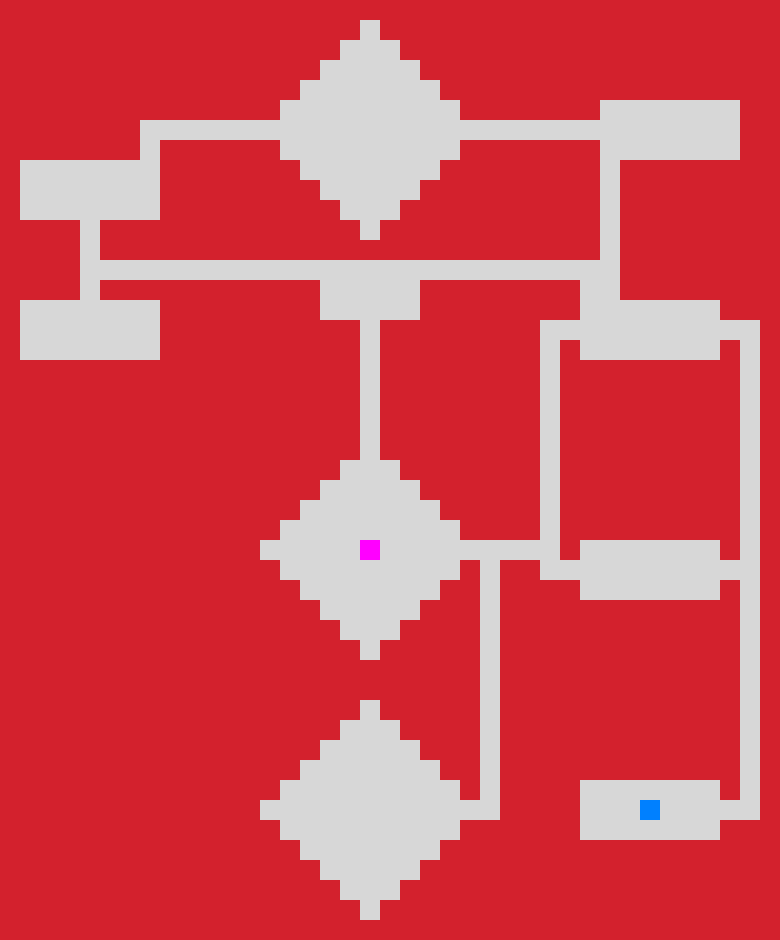
\includegraphics[width=0.5\textwidth]{Images/p1t1_start.png}
        \caption[Task 1 startgrid]{Task 1 grid with start and end points.}
        \label{fig:Task 1 startgrid}
    \end{figure}

    \begin{figure}[H]
        \centering
        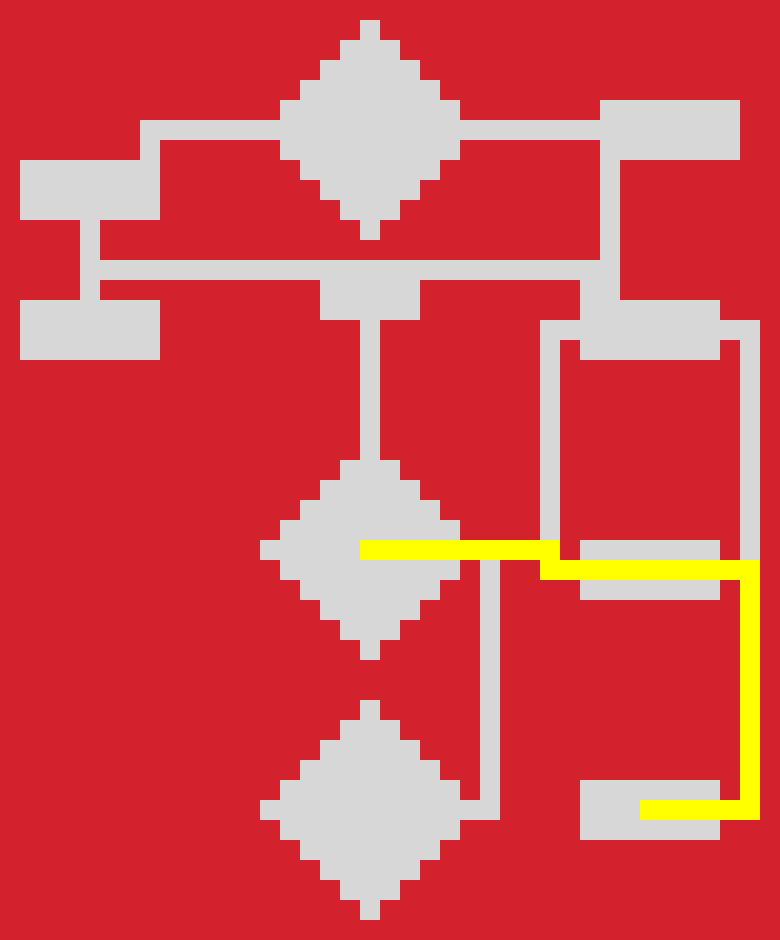
\includegraphics[width=0.5\textwidth]{Images/t1p1_finish.png}
        \caption[Task 1 endgrid]{Task 1 grid with visualization of the shortest path.}
        \label{fig:Task 1 endgrid}
    \end{figure}

    \newpage

    \textbf{Task 2}

    \begin{figure}[H]
        \centering
        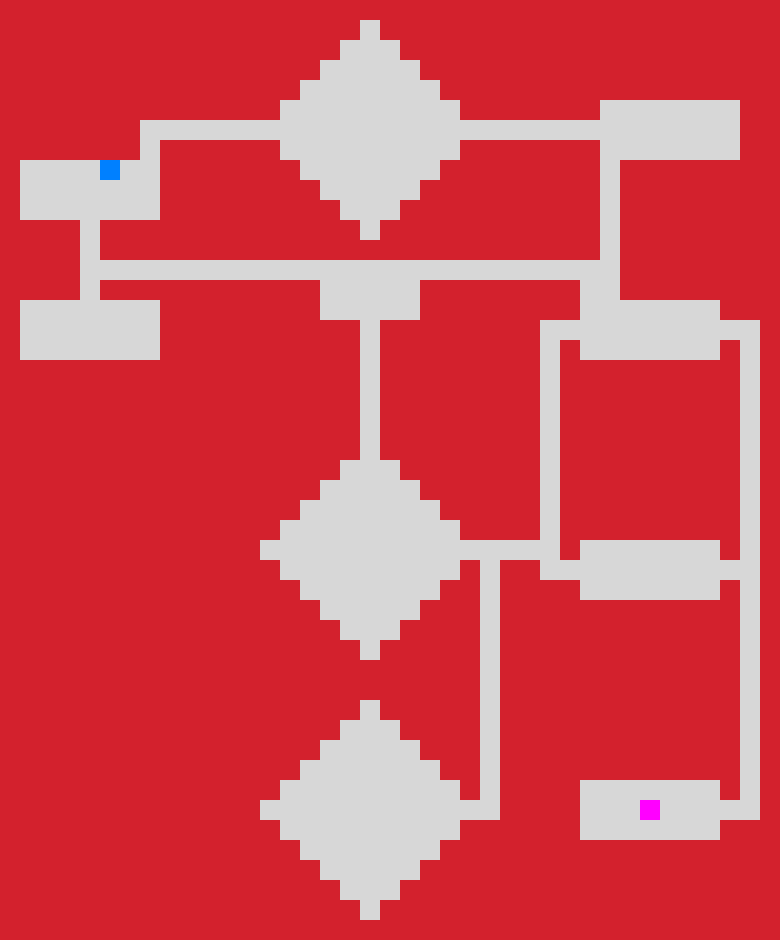
\includegraphics[width=0.5\textwidth]{Images/p1t2_start.png}
        \caption[Task 1 startgrid]{Task 2 grid with start and end points.}
        \label{fig:Task 2 startgrid}
    \end{figure}

    \begin{figure}[H]
        \centering
        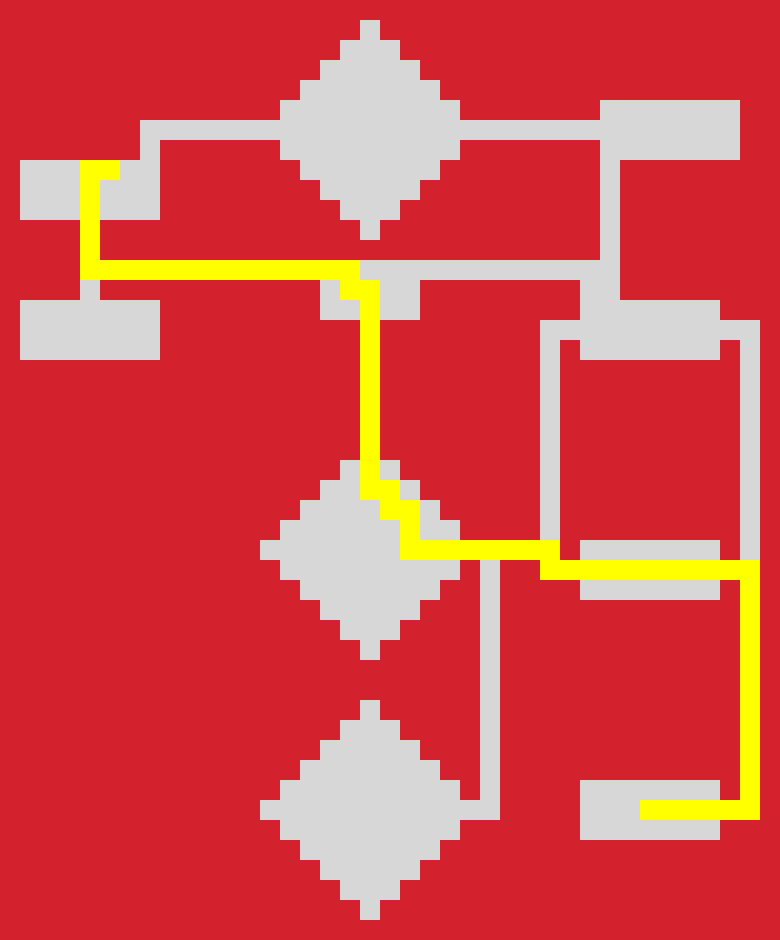
\includegraphics[width=0.5\textwidth]{Images/p1t2_finish.png}
        \caption[Task 1 endgrid]{Task 2 grid with visualization of the shortest path.}
        \label{fig:Task 2 endgrid}
    \end{figure}

    \newpage

    \section*{Part 2}

    \textbf{Task 3}

    \begin{figure}[H]
        \centering
        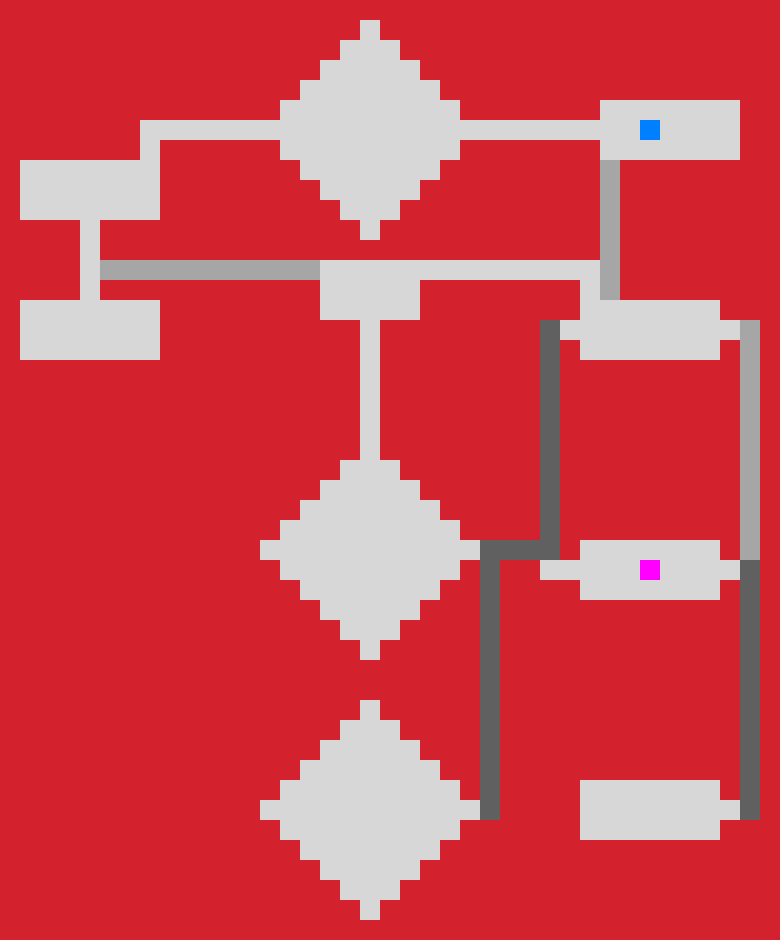
\includegraphics[width=0.5\textwidth]{Images/p2t3_start.png}
        \caption[Task 1 startgrid]{Task 3 grid with start and end points.}
        \label{fig:Task 3 startgrid}
    \end{figure}

    \begin{figure}[H]
        \centering
        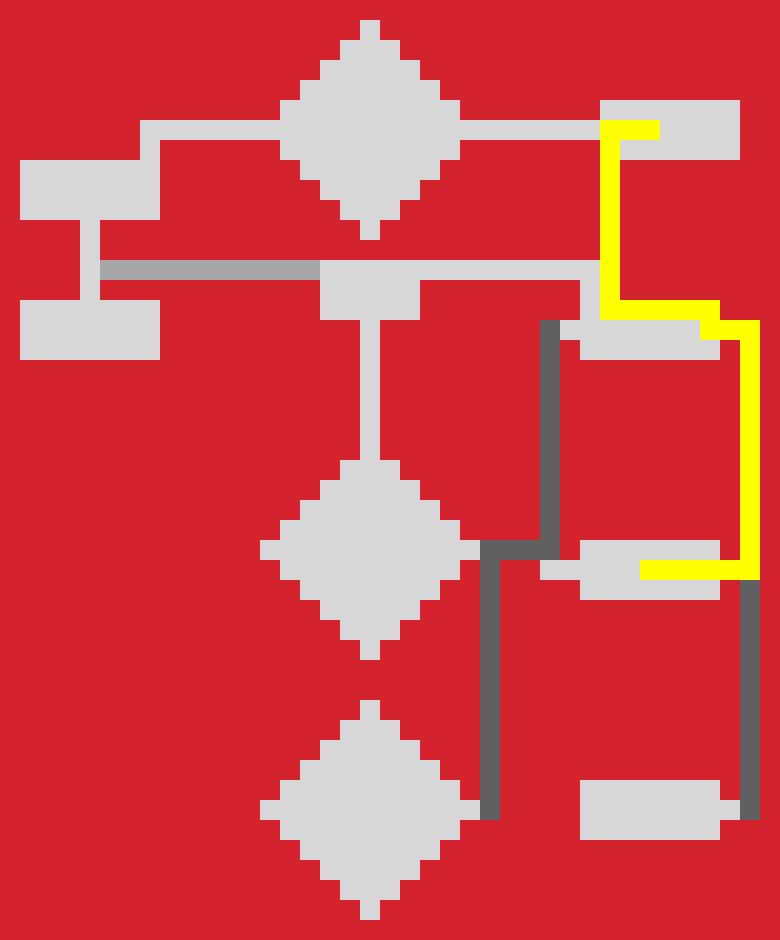
\includegraphics[width=0.5\textwidth]{Images/p2t3_finish.png}
        \caption[Task 1 endgrid]{Task 3 grid with visualization of the shortest path.}
        \label{fig:Task 3 endgrid}
    \end{figure}

    \newpage

    \textbf{Task 4}

    \begin{figure}[H]
        \centering
        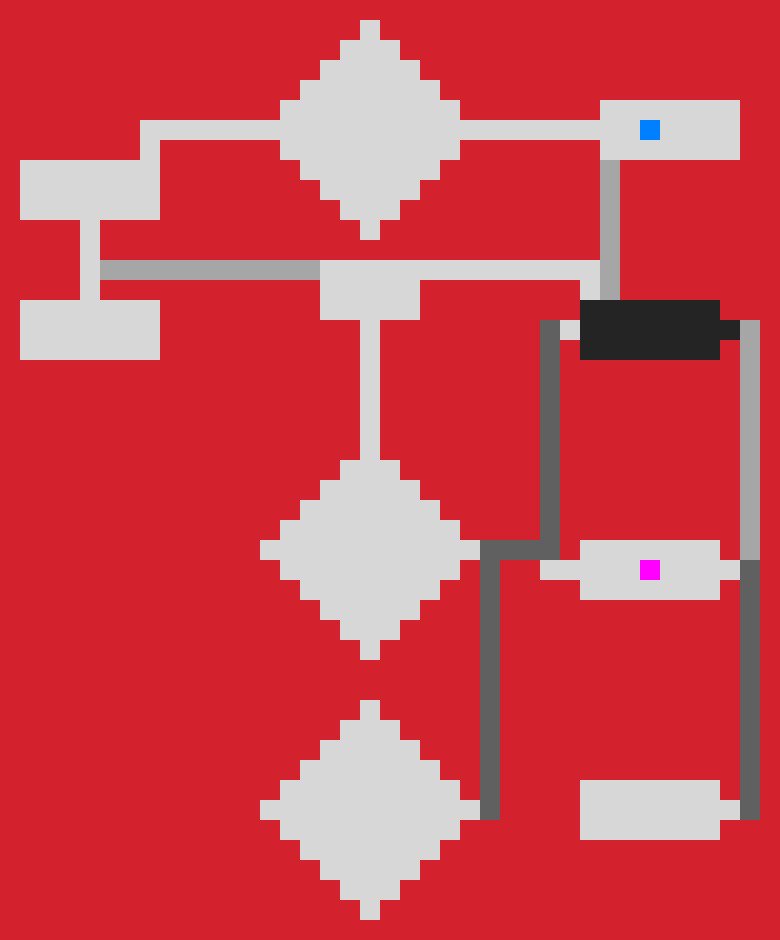
\includegraphics[width=0.5\textwidth]{Images/p2t4_start.png}
        \caption[Task 1 startgrid]{Task 4 grid with start and end points.}
        \label{fig:Task 4 startgrid}
    \end{figure}

    \begin{figure}[H]
        \centering
        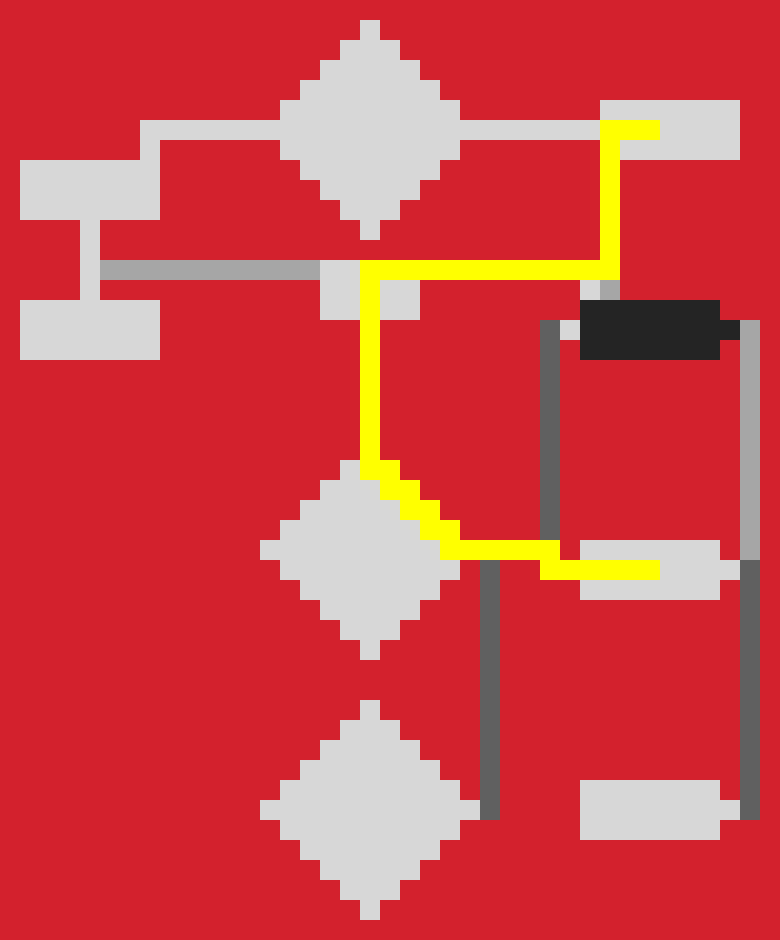
\includegraphics[width=0.5\textwidth]{Images/p2t4_finish.png}
        \caption[Task 1 endgrid]{Task 4 grid with visualization of the shortest path.}
        \label{fig:Task 4 endgrid}
    \end{figure}

% End of document
\end{document}
